\chapter{Introduction}
\label{cha:introduction}

Additive manufacturing or AM (most commonly known as 3D printing) is the process of constructing a three-dimensional object
by means of depositing material (usually layer by layer) onto the object in order to achieve a desired shape.

The origins of this technology dates back to the 1980s, with the real ``3D Printer'' being created by Hideo Kodama, and described
in his paper ``Automatic method for fabricating a three‐dimensional plastic model with photo‐hardening polymer'' \cite{am_origins}.
During the 2000s 3D printing remained a fairly expensive process, with it's use being limited for prototyping inside of companies
that could afford it. A turning point in the history of the technology came in 2009, when the Fused Deposition Modeling (FDM) printing process 
patents expired, allowing many startups to ender the game.
In the following years, as the technology matured it become clear that 
AM could be used for more that prototyping, and some companies started leveraging its unique advantages in actual production lines.
One of the first industry to successfully integrate this technology in it's supply chain was the aviation sector,
where the ability to create higgle complex shapes is extraordinary helpful to reduce weight of various components.

While the technology was establishing a footprint in the manufacturing world, a separate innovation was happening on the side:
RepRap (Replicating Rapid Prototyper) \cite{reprap} was a project developed in the University of Bath, that aimed 
to develop an open source 3D printer that was cheap to produce.
The project was widely regarded as a success, and managed to build approximately 4500 machines in 2 and a half years.

In 2012 Prusa Research was founded and the company started selling it's famous i3 model \cref{fig:prusa_i3} (that was based on the RepRap project)
at a starting price of approximately €600. Since then consumer 3D printers have only become better and cheaper thanks to companies
such as Creatily, Elegoo and BambooLab.
\cite{print_pictures}



\begin{figure}[h]
    \centering
    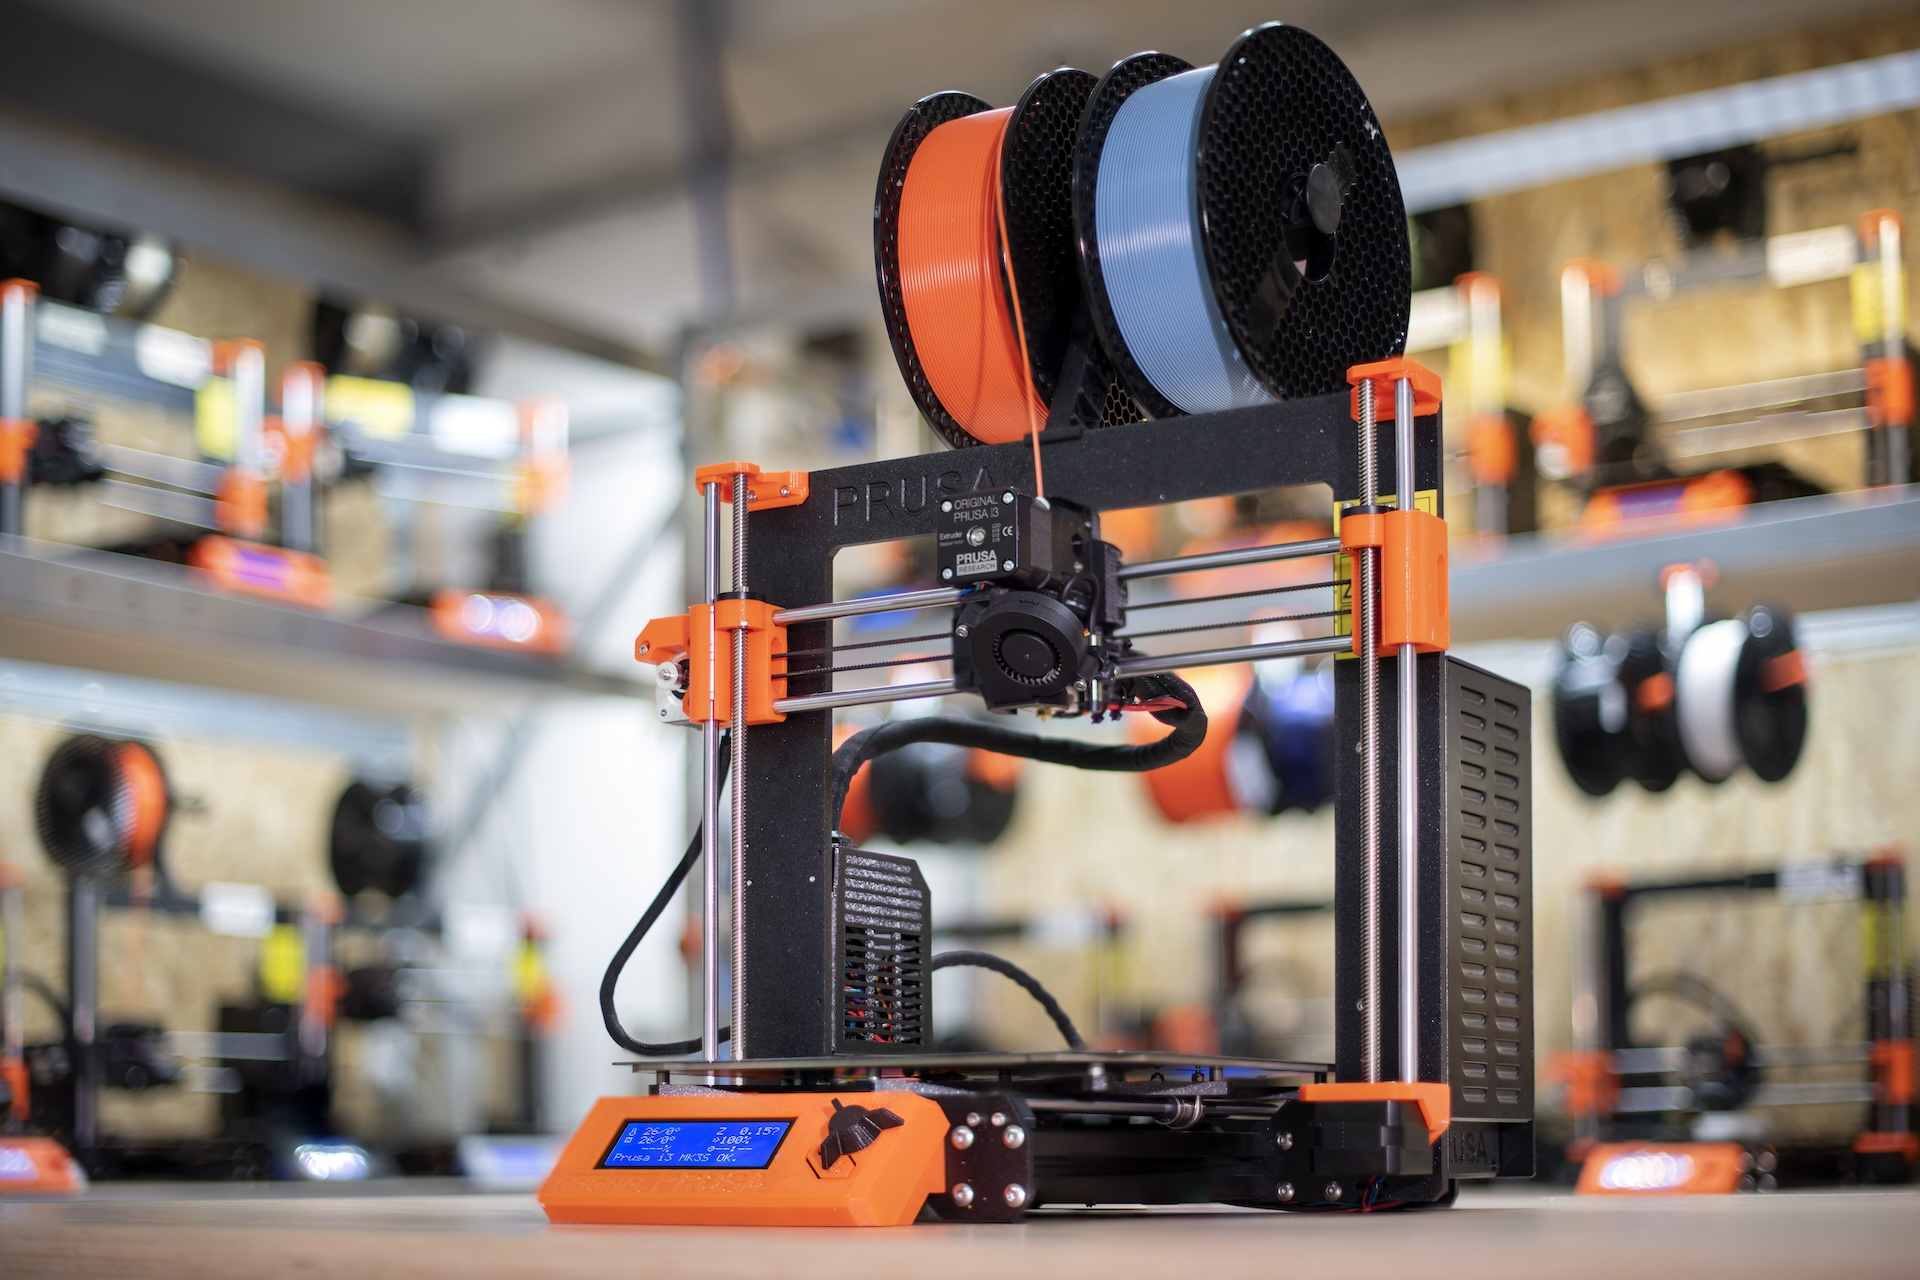
\includegraphics[width=0.33\textwidth]{images/prusa_i3.png}
    \caption{Original Prusa i3 Printer}
    \label{fig:prusa_i3}
\end{figure}


\section{3D printing technologies}

It is worth mentioning that the therm ``Additive manufacturing'' is a broad term that includes widely different techniques, each of them
has it's own strength and weaknesses. This section is not meant to be a comprehensive survey of all the 3D printing technologies, 
instead we will give a brief overview of the three most important techniques, and we will mention the advantages and disadvantage
of each of them, with a special focus on the forces that are applied on the printed object while it's being manufactured, which is
a factor that is particularly relevant for this thesis.

\noindent The techniques that we will explain in this section are:
\begin{itemize}
    \item Fused Deposition Modeling (FDM)
    \item Stereophotography (SLA)
    \item Selective Laser Sintering (SLS)
\end{itemize}
It is worth noting that an actual topology of 3D printing technologies is much more complicated than this simple list, however
the level of detail provided in this introduction is more than enough to understand the work presented in this thesis.

\subsection{Fused Deposition Modeling (FDM)}

Fused Deposition Modeling (FDM) is a technique that relies on a thermoplastic filament— that is fed by an extruder into a heated nozzle.
This nozzle melts the filament and moves through 3D space using a set of at least three motors.
To control this movement, a software program called a ``slicer'' converts a 3D model into a set of instructions known as ``gcode.''
These instructions are then processed by the printer's controller, guiding the nozzle to deposit the material layer by layer 
until the final object is created.


\begin{figure}[h]
    \centering
    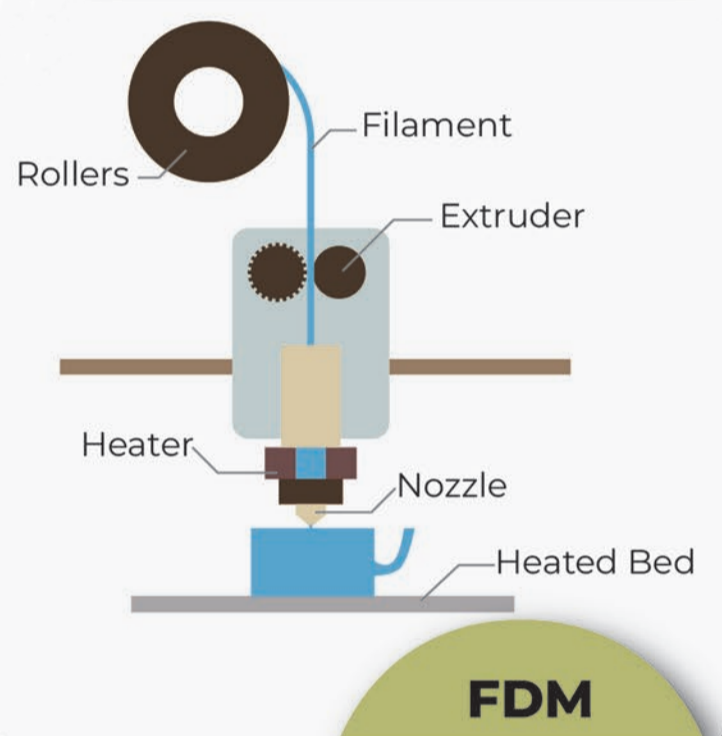
\includegraphics[width=0.33\textwidth]{images/fdm.png}
    % \caption{FDM technology overview (source: Martins 2023 \cite{print_pictures})}
    \caption[FDM technology overview.]{FDM technology overview (source: Martins 2023 \cite{print_pictures})}
    \label{fig:fdm}
\end{figure}

FDM is currently the most common 3D printing techniques for ``hobbyist'', as it's the cheapest option available, 
have good print dimensions (with most 3D printer having a build volume of 256x256x256mm).
Another advantage of FDM printing is the wide variety of usable materials, some of them (like PLA) are cheap,
and easy to print, others like ABS are more durable. Then there are a series of exotic material that offer
specific features, for example TPU is a material that is flexible and allow to print soft surfaces, while PVA
is a material solvable in water and is often used to print supports that can be removed simply by submerging
the printed object in water.
Another feature that is exclusive to FDM printer is the ability to print with multiple materials,
this is done with either a mechanism that automatically switch the filament used, or with printers that
have multiple nozzles.



\subsection{Stereophotography (SLA)}

\begin{figure}[h]
    \centering
    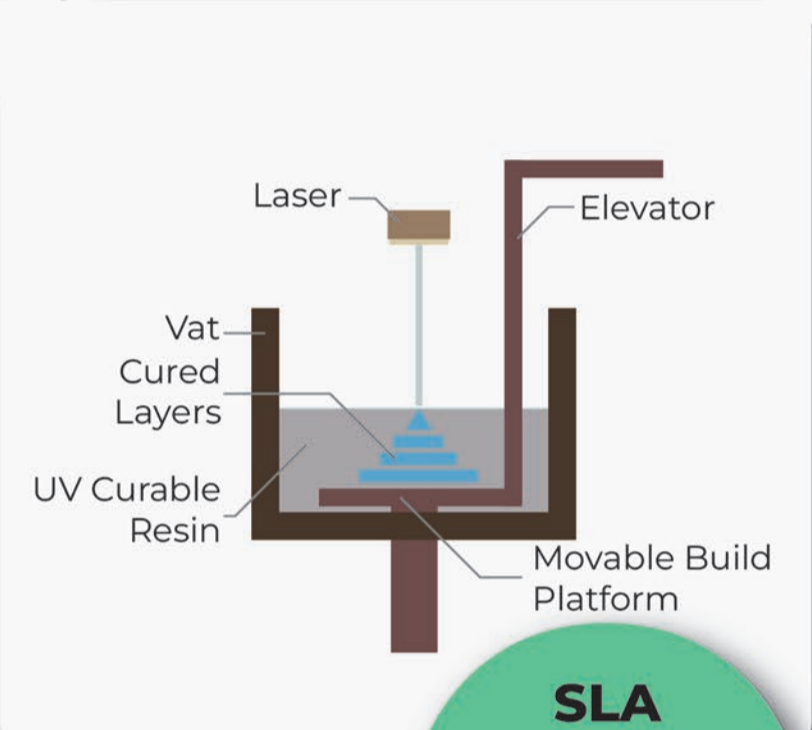
\includegraphics[width=0.33\textwidth]{images/sla.png}
    \caption{SLA technology overview (source: Martins 2023 \cite{print_pictures})}
    \label{fig:sla}
\end{figure}
Fused Deposition Modeling (or FDM for short)


\subsection{Selective Laser Sintering (SLS)}

\begin{figure}[h]
    \centering
    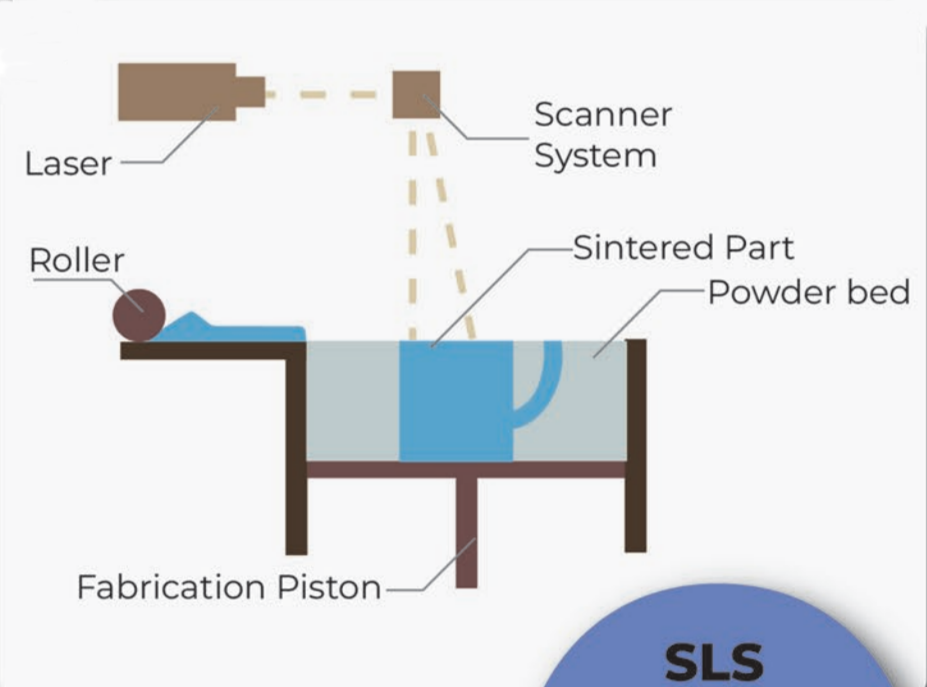
\includegraphics[width=0.33\textwidth]{images/sls.png}
    \caption{SLS technology overview (source: Martins 2023 \cite{print_pictures})}
    \label{fig:sla}
\end{figure}
Fused Deposition Modeling (or FDM for short)



